% !TeX root = ./document.tex
\documentclass[document]{subfiles}
\begin{document}

\chapter{Спектр и резольвента оператора}

\begin{definition}
    $X$ --- банахово, $T \in \B(X), Ix = x, x \in X$ --- тождественный оператор
    \[ \lambda \in \bC \quad V(\lambda) : \bC \rightarrow \B(X) \quad V(\lambda) = \lambda I - T \]
    Теперь множество комплексных чисел разбивается на 2 подмножества. $\lambda$ --- \textbf{регулярное значение}, если $V(\lambda)$ --- биекция [[ теорема Банаха ]] $\Rightarrow
    \: \exists (V(\lambda))^{-1} \in \B(X)$. 

    $\rho(T) = \{ \lambda \text{ --- регулярная } \}$ --- \textbf{резвольвентное множество}
    \[ R(\lambda) : \rho(T) \rightarrow \B(X) \quad \R(\lambda, T) = R(\lambda) = (V(\lambda))^{-1} \]
    $R$ --- \textbf{резольвента}
\end{definition}

Операторо-значная функция: комплексному числу сопоставляем оператор.

Откуда берется такое пугающее слово резольвента? Рассмотрим уравнение $\lambda x - Tx = y$. Если $\forall y \in X \exists! x$ --- решение этого уравнения, 
то $\lambda$ --- регулярное значение, а уравнение --- разрешимо (resolve). Англо-саксонское слово проникло и сюда

\[ \sigma(T) = \bC \setminus \rho(T)  \text{ --- спектр оператора }\]

Посмотрим, из каких частей состоит этот спектр. Почему $V$ может быть не биекцией? В конечномерных пространствах он мог быть только не инъекцией, но в бесконечномерных 
может быть и не сюръекцией.

\begin{enumerate}
    \item $\sigma_p$ --- точечный спектр (p = point)
    \begin{gather*}
        \lambda \in \sigma_p(T) \text{ если } \Ker(\lambda I - T) \ne \seq{0} \\
        X_\lambda = \Ker(\lambda I - T), x \in X_\lambda \Leftrightarrow Tx = \lambda x
    \end{gather*}
        $\lambda$ --- собственное значение, $X_\lambda$ --- собственное подпространство 
    \item $\sigma_c(T)$ --- непрерывный спектр (c = continuous) 
    \begin{gather*}
        \sigma_c(T) = \seq{\lambda \in \bC, \Ker(\lambda I - T) = \seq{0}} \\
        V(\lambda) \text{ --- всюду плотен в } X, \text{ то есть } \overline{(\lambda I - T)(X)} = X
    \end{gather*}
    хоть и не биекция, но почти --- на всюду плотном множестве существует решение уравнения
    \item $\sigma_r(T)$ --- остаточный спектр (r = reminder)
           \[ \sigma_r = \seq{\lambda \in \bC: \Ker(\lambda I - T) = \seq{0}, \overline{\lambda I - T}(X) \subsetneq X } \] 
           образ $(V(\lambda))(X)$ не плотен в $X$
\end{enumerate}

\[ \sigma(T) = \sigma_p(T) \cup \sigma_c(T) \cup \sigma_r(T) \] 
части спектра не пересекаются

\begin{example}
    Если $\dim X < +\infty$, то $\sigma(T) = \sigma_p(T)$
\end{example}

\begin{theorem}[свойства резольвенты]
    $X$ --- банахово, $T \in \B(X), \: \lambda, \mu \in \rho(T)$
    \begin{enumerate}
        \item $R(\lambda) R(\mu) = R(\mu) R(\lambda)$
        \item $R(\lambda)-R(\mu)=(\mu-\lambda)R(\lambda)R(\mu)$ (тождество Гильберта) 
        \item $\lambda \in \bC. \abs{\lambda} \geq \norm{T} \Rightarrow \lambda \in \rho(T)$
        \item $\rho(T)$ --- открытое множество, $\mu \in \rho(T), \seq{\lambda \in \bC: \abs{\lambda - \mu} < \frac{1}{\norm{R(\mu)}}} \subset \rho(T)$
        \item $R(\lambda)$ --- непрерывная функция, то есть $\liml_{\lambda \to \mu} \norm{R(\lambda) - R(\mu)} = 0, \liml_{\lambda \to \infty} R(\lambda) = 0$
        \item $F \in (\B(X))^*, g(\lambda) = F(R(\lambda)), \lambda \in \rho(T) \Rightarrow g(\lambda)$ --- аналитическая в $\rho(T)$ (то есть $\exists g^\prime(\lambda))$
    \end{enumerate}
\end{theorem}

\begin{proof}[1]
    \begin{gather*}
        V(\lambda)V(\mu) = (\lambda I - T)(\mu I - T) = (\mu I - T)(\lambda I - T) = V(\mu)V(\lambda) \\
        AB = BA, \: A,B \in \B(X), \: \exists A^{-1}, B^{-1} \Rightarrow \\
        (AB)^{-1} = (BA)^{-1} \Leftrightarrow B^{-1}A^{-1} = A^{-1}B^{-1}
    \end{gather*}
\end{proof}

\begin{proof}[2]
    \begin{gather*}
        A^{-1} - B^{-1} = A^{-1}(B-A)B^{-1} \\
        A = V(\lambda) = \lambda I - T \quad B = V(\mu) = \mu I - T \\
        B - A = (\mu - \lambda) I \\
        \Rightarrow R(\lambda) - R(\mu) = R(\lambda)(\mu - \lambda)I \cdot R(\mu) = (\mu - \lambda)R(\lambda)R(\mu)
    \end{gather*}
    это рассужедние связано с утвержедниями об открытости множества обратимых операторов, об обратимости оператора, близкого к тождественному,
     и всё это мы будем сейчас использовать
\end{proof}

\begin{proof}[3]
    \begin{gather*}
        \lambda \in \bC, \abs{\lambda} > \norm{T} \\
        V(\lambda) = \lambda I - T = \lambda \left(I - \frac{1}{\lambda} T \right)
        \norm{\frac{1}{\lambda} T} < 1 \\
         [[\text{ теорема об обратимости оператора, близкого к тождественному }]] \Rightarrow \\
        \exists \left( I - \frac{1}{\lambda}T \right)^{-1} \Rightarrow R(\lambda) = \frac{1}{\lambda} \left(I - \frac{1}{\lambda}T \right)^{-1}
    \end{gather*}
\end{proof}

\begin{proof}[4]
    \begin{gather*}
        A \in \In(X), \text{ то есть } A \text { обратим}, [[\text{ теорема об открытости } \In(X)]] \Rightarrow \\ 
        \norm{B-A} < \frac{1}{\norm{A^{-1}}} \Rightarrow B \in \In(X) \\
        A = \mu I - T \quad B = \lambda I - T \\
        \norm{A - B} = \abs{\lambda - \mu} \quad \abs{\lambda - \mu} < \frac{1}{\norm{R(\mu)}} \Rightarrow \: \exists B^{-1}, \text{ т.е. } R(\lambda), \text{ т.е. } \\
        \lambda \in \rho(T)
    \end{gather*}
\end{proof}

\begin{proof}[5]
    \begin{gather*}
        \norm{V(\lambda) - V(\mu)} = \abs{\lambda - \mu} \\
        \liml_{\lambda \to \mu} \norm{V(\lambda) - V(\mu)} = 0 \\
        \varphi : \In(X) \rightarrow \In(X) \quad \varphi(A) \coloneqq A^{-1} 
        \intertext{$\varphi$ --- непрерывное отображение, доказали в теореме об открытости $\In(X)$} 
        \Rightarrow \liml_{\lambda \to \mu} \varphi(V(\lambda)) = \varphi(V(\mu)) \Leftrightarrow \liml_{\lambda \to \mu} R(\lambda) = R(\mu) \\
        \liml_{\lambda \to \infty} \frac{1}{\lambda} T = 0 \Rightarrow \liml_{\lambda \to \infty} \left(I - \frac{1}{\lambda} T \right) = I [[\text{ непрерывности } \varphi]] \Rightarrow \\
        \liml_{\lambda \to \infty} \left(I - \frac{1}{\lambda} T \right)^{-1} = I \Rightarrow \liml_{\lambda \to \infty} R(\lambda) = \liml_{\lambda \to \infty} \frac{1}{\lambda} \left(I- \frac{1}{\lambda}T\right)^{-1} = 0 \\
        R(\lambda) = \frac{1}{\lambda} \left(I - \frac{1}{\lambda} T \right)^{-1}
    \end{gather*}
\end{proof}

\begin{proof}[6]
    \begin{gather*}
        \frac{R(\lambda)-R(\mu)}{\lambda - \mu} \stackrel{2}{=} \frac{(\mu-\lambda)R(\lambda)R(\mu)}{\lambda - \mu} = -R(\lambda) R(\mu) \underset{\lambda \to \mu}{\longrightarrow} - R(\mu)^2
        %\intertext{можно было бы сказать, ура, есть аналитическая функция со значениями в банаховом пространстве, но у нас пока его нет}
        F \in (\B(X))^* \quad g(\lambda) = F(R(\lambda)) \\
        \frac{g(\lambda) - g(\mu)}{\lambda - \mu} = \frac{F(R(\lambda)) - F(R(\mu))}{\lambda - \mu} = F \left( \frac{R(\lambda) - R(\mu)}{\lambda - \mu} \right) \underset{\lambda \to \mu}{\longrightarrow} \\
        -F((R(\mu))^2) \Rightarrow \: \exists g^\prime(\mu) \: \forall \mu \in \rho(T)
    \end{gather*}
\end{proof}

Важная теорема, которая будет простым следствием из доказанных свойств

\begin{theorem}[компактность и не пустота спектра]
    $X$ --- банахово, $T \in \B(X) \Rightarrow \sigma(T)$ --- не пуст и компактен
\end{theorem}

Достаточно необычно, что для того, чтобы показать непустоту спектра, нам понадобится ТФКП, математика всё-таки едина, ёлы-палы! 
\begin{theorem}[Лиувилль]
    Пусть $f(\lambda)$ --- аналитическая в $\bC$ и ограниченная, то есть $\exists M  > 0 : \abs{f(\lambda)} \leq M \: \forall \lambda \in \bC \Rightarrow f(\lambda) \equiv const$.
\end{theorem}

По секрету, функции, аналитические во всей комплексной плоскости, называются \textbf{целыми}.
\begin{proof}[Доказательство теоремы Лиувилля]
    \begin{gather*}
        a \in \bC \quad f^\prime(a) = \frac{1}{2\pi} \int_{\seq{|z-a| = r}} \frac{f(z)}{(z-a)^2} dx \Rightarrow
        \intertext{то есть продифференцировали формулу Коши. Когда функция у нас целая, мы $r$ можем взять любое}
        \Rightarrow \abs{f^\prime(a)} \leq \frac{1}{2\pi} \frac{M \cdot 2\pi r}{r^2} = \frac{M}{r} \underset{r \to \infty}{\longrightarrow} 0 \\
        \Rightarrow f^\prime(a) = 0 \: \forall a \in \bC \\
        \Rightarrow f(\lambda) = c \: \forall \lambda \in \bC, c \in \bC
    \end{gather*}
\end{proof}

\begin{figure}
    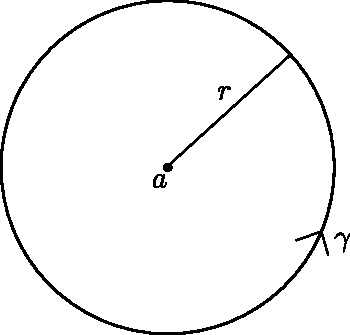
\includegraphics{chapter11/liuvill.pdf}\caption{Теорема 11.3}
\end{figure}

\begin{proof}[Доказательство теоремы]
    $\rho(T)$ --- открыто, $\rho(T) \subset \bC \Rightarrow \sigma(T) = \bC \setminus \rho(T)$ --- замкнутое. 
    \[ \abs{\lambda} > \norm{T} \Rightarrow \lambda \subset \rho(T) \Rightarrow \sigma(T) = \seq{\lambda \in \bC: \abs{\lambda} \leq \norm{T}} \text{ --- ограниченное} \]
    $\Rightarrow \sigma(T)$ --- компакт.

    \begin{gather*}
        \text{пусть } \sigma(T) \ne \varnothing \Rightarrow \rho(T) = \bC \Rightarrow 0 \in \rho(T) \\
        V(0) = 0 \cdot I - T = -T, 0 \in \rho(T) \Rightarrow \: \exists T^{-1} \\
        \exists F \in (\B(X))^* : F(T^{-1}) = \norm{T^{-1}}, F(T^{-1}) \ne 0 \\
        g(\lambda) = F(R(\lambda)) \quad g(0) \ne 0, 6 \text{ свойство } \Rightarrow g(\lambda) \text{ аналитическая в } \bC  \\ 
        \liml_{\lambda \to \infty} R(\lambda) = 0 \Rightarrow \liml_{\lambda \to \infty} g(\lambda) = \liml_{\lambda \to \infty} F(R(\lambda)) = 0 \\
        [[\exists R > 0: \abs{g(\lambda)} \leq 1 \text{ при } \lambda \geq R, \exists M = \max_{|\lambda| \leq \bR} \abs{g(\lambda)} \Rightarrow \abs{g(\lambda)} \leq \max \{1, \mu \}]]
        \intertext{применяем теорему Лиувилля}
        g(\lambda) = const, \liml_{\lambda \to \infty} g(\lambda) = 0  \Rightarrow g(\lambda) \equiv 0 \Rightarrow g(0) = 0\\
        \text{противоречие } \Rightarrow \sigma(T) \ne \varnothing
    \end{gather*}
\end{proof}

\begin{definition}[Спектральный радиус оператора $T$]
    $r(t) = \max_{\lambda \in \sigma(T)} \abs{\lambda}$. Из теоремы $\Rightarrow r(T) \leq \norm{T}$
\end{definition}
Примем без доказательства формулу
\[ r(T) = \liml_{n \to \infty} \sqrt[n]{\norm{T^n}} \] 

Наконец, обсудим, как связаны между собой спектр оператора и спектр сопряженного оператора.

\begin{theorem}[спектр сопряженного оператора]
    \begin{enumerate}
        \item $X$ --- банахово, $T \in \B(X) \Rightarrow$
            \begin{gather*}
                \sigma(T^*) = \sigma(T) \\
                \lambda \in \rho(T) \Rightarrow (R(\lambda, T))^* = R(\lambda, T^*)
            \end{gather*}
        \item $H$ --- гильбертово, $T \in \B(H), T^*$ --- эрмитово сопряженный 
            \begin{gather*}
                \sigma(T^*) = \seq{\overline{\lambda} : \lambda \in \sigma(T)} \\
                \lambda \in \rho(T) \quad R(\overline{\lambda}, T^*) = (R(\lambda, T))^*
            \end{gather*}
    \end{enumerate}
\end{theorem}

\begin{proof}[1]
    \begin{gather*}
        \left. \begin{matrix}
            \text{пусть } \lambda \in \rho(T) \Rightarrow \: \exists (\lambda I - T)^{-1} \\
            (\lambda I - T)^* = \lambda I - T^*
        \end{matrix} \right\} \Rightarrow \: \exists (\lambda I - T^*)^{-1} = ((\lambda I - T)^{-1})^*
    \end{gather*}
    В обратную сторону по замечанию из начала лекции %ссылку
\end{proof}

\begin{proof}[2]
    \[ (\lambda I - T)^* = \overline{\lambda} I - T^* \text{ и так далее} \]
\end{proof}

Маленькое ДЗ, которое когда-то давали в качестве задачи на 5 на экзамене
\begin{statement}
    $H$  --- гильбертово, $M$ --- замкнутое подпространство. $P : H \rightarrow M$ --- ортопроектор. $\sigma(P), R(\lambda)$ = ?
\end{statement}

Иногда кровожадные помощники задавали такие вопросы (но это не на 5, это просто на 1 секунду подумать): $I$ --- тождественный, $\sigma(I)$ = ?

\section{Компактные операторы}

\begin{definition}[компактный оператор]
    $X,Y$ --- банаховы, $T \in \Lin(X,Y)$. $T$ --- компактный, если $T(B^X_1(0))$ --- относительно компактен
\end{definition}

$\Com(X,Y)$ --- множество всех компактных операторов. Если $X=Y$, будем писать $\Com(X)$

\begin{remark}
    $\Com(X,Y) \subset \B(X,Y)$, $T(B^X_1(0))$ --- относительно компактно $\Rightarrow$ $(T(B^X_1(0))) \Rightarrow T(B^X_1(0))$ --- ограниченное $\Rightarrow T \in \B(X, Y)$
\end{remark}

\begin{remark}
    $\forall A \subset X, A$ --- ограниченное, $T \in \Com(X,Y) \Rightarrow T(A)$ --- относительно компактно
\end{remark}


Теперь еще один способ сказать, что оператор --- компактный. 
\begin{remark}
    $T \in \Com(X,Y) \Leftrightarrow \: \forall \seq{x_n}^\infty_{n=1} \text{ --- ограниченная } \Rightarrow \: \exists \seq{n_k}^\infty_{k=1} \text{ т. ч. } \exists \liml_{k \to \infty} T(x_{n_k}) = y_0 \in Y$
\end{remark}

Более узкий класс операторов, но они же являются и примерами компактных операторов:
\begin{definition}[оператор конечного ранга]
    $X,Y$ --- банаховы, $T \in \B(X,Y), T$ --- \textbf{оператор конечного ранга}, если $\dim(T(X)) < +\infty$
\end{definition}

\begin{example}
    \begin{gather*}
        \seq{y_j}^n_{j=1}, y_j \in Y, \seq{f_j}^n_{j=1}, f_j \in X^* \\
        x \in X \quad Tx = \sum^n_{j=1} f_j(x) y_j \\
        \rank T = n
    \end{gather*}
\end{example}

Небольшое  ДЗ: показать, что оператор конечного ранга имеет такой вид.

\begin{statement}
    $T$ --- оператор конечного ранга $\Rightarrow T \in \Com(X, Y)$
\end{statement}

\begin{proof}
    $\dim(T(X)) < +\infty, T \in \B(X,Y) \Rightarrow T(B^X_1(0))$ --- ограниченное множество в конечномерном пространстве
     $\Rightarrow T(B^X_1(0))$ --- относительно компактно
\end{proof}

Существенная теорема о том, как связаны между собой компактность, операторы конечного ранга, конечномерные подпространства.

\begin{theorem}
    $X,Y$ --- банаховы, $T \in \Com(X,Y)$. Если $L = \overline{L}, L$ --- подпространство $T(X) \Rightarrow \dim L < +\infty$
\end{theorem}

\begin{proof}
    Первая часть доказательства. Допустим, что $L = T(X)$. Иными словами, предполагаем, что образ замкнут $\Rightarrow T(X)$ --- банахово. Тогда вот что у нас есть
    \begin{gather*}
        T: X \rightarrow T(X) [[\text{ теорема Банаха об открытом отображении }]] \Rightarrow \\
        \exists B_r^{T(X)}(0) \subset T(B^X_1(0)) \text{ --- относительно компактно} \\
        \Rightarrow B_r^{T(X)}(0) \text{ --- относительно компактно} \\
        [[\text{ теорема Рисса }]] \dim(T(X)) < +\infty
    \end{gather*}
    Вторая часть, и тут другая идея, как это свестии к предыдущему пункту. Рассмотрим $X_1 = T^{-1}(L), X_1$ --- банахово 
    \[ T(X_1) = L, T \in \Com(X_1, L) \stackrel{1}{\Rightarrow} \dim L < +\infty \]
\end{proof}

\begin{corollary}
    $X$ --- банахово, $T \in \Com(X)$
    \begin{enumerate}
        \item Если $T(X) = X$, то $\dim X < +\infty$ 
        \item Если $\dim X = +\infty$, то $0 \in \sigma(T)$
    \end{enumerate}
\end{corollary}

\begin{proof}
    Первое очевидно. Второе:

    \begin{gather*}
        0 \in \rho(T) \Leftrightarrow V(0) = 0 \cdot I - T = -T, \: \exists T^{-1} \Rightarrow T(X) = X \text{ --- противоерчие с 1} \\
        \Rightarrow 0 \in \sigma(T)
    \end{gather*}
\end{proof}

Посмотрим теперь, какие арифметические операции можно выполнять с компактными операторами

\begin{theorem}[арифметические операции и предельный переход в $\Com(X,Y)$]
    $X,Y$ --- банаховы 
    \begin{enumerate}
        \item $\Com(X,Y)$ --- замкнутое подпространство в $\B(X,Y)$. Поэтому будет сложение, композиция, умножение на константу и переход к пределу 
        \item $X \stackrel{T}{\rightarrow} Y \stackrel{S}{\rightarrow} Z, \: X, Y, Z$ --- банаховы
            \begin{enumerate}
                \item $T \in \B(X,Y), S \in \Com(Y,Z) \Rightarrow ST \in \Com(X,Z)$
                \item $T \in \Com(X,Y), S \in \B(Y,Z) \Rightarrow ST \in \Com(X,Z)$
            \end{enumerate}
    \end{enumerate}
\end{theorem}

\begin{proof}[1]
    \begin{gather*}
        T \in \Com(X,Y), \alpha \in \bC [[\text{ очевидно }]] \Rightarrow \alpha T \in \Com(X, Y) \\
        T, S \in \Com(X,Y) \quad B = B^X_1(0)
        \intertext{вспомним, что в полном пространстве относительная компактность эквивалентна вполне ограниченности}
        T(B) \text{ --- относительно компактно } \Leftrightarrow \text{ вполне ограничено} \\
        \varepsilon > 0 \: \exists E \text{ --- конечная } \varepsilon\text{-сеть для } T(B) \\  
        \exists F \text{ --- конечная } \varepsilon\text{-сеть для } S(B) \\
        E + F = \seq{e + f : e \in E, f \in F} \text{ --- конечная } 2\varepsilon\text{-сеть для множества } T(B) + S(B) \\
        (T+S)(B) \subset T(B) + S(B) \\ 
        \Rightarrow (T+S)(B) \text{ --- вполне ограничено } \Rightarrow \text{ относительно компактно}
    \end{gather*}
    Проверим замкнутость $\Com(X,Y)$. Возьмём 
    \begin{gather*}
        \seq{T_n}^\infty_{n=1}, T_n \in \Com(X,Y) \\
        \liml_{n \to \infty} \norm{T_n - T} = 0
        \intertext{опять-таки воспользуемся вполне ограниченностью}
        \text{пусть } \varepsilon > 0 \: \exists n \in \bN : \norm{T_n - T} < \varepsilon \\
        \exists E \text{ --- конеченая } \varepsilon\text{-сеть для } T_n(B) \\
        \Rightarrow E \text{ --- } 2\varepsilon{-сеть для} T(B) \Rightarrow T(B) \text{ --- вполне ограничено}
    \end{gather*}
\end{proof}

\begin{proof}[2]
    $X \stackrel{T}{\rightarrow} Y \stackrel{S}{\rightarrow} Z, B = B^X_1(0)$

    Первый пункт: $T \in \B(X,Y) \Rightarrow T(B)$ --- ограниченное множество $\Rightarrow S(T(B))$ --- относительно компактно.

    Второй пункт: $T \in \Com(X,Y) \Rightarrow T(B)$ --- относительно компактен. $S$ --- непрерывное отображение $\Rightarrow S(T(B))$ --- относительно компактно.
\end{proof}

Вот какую умность можно сказать:
\begin{corollary}
    $X$ --- банахово, $\Com(X)$ --- замкнутый двусторонний идеал алгебры $\B(X)$
\end{corollary}

\section{Спектр компактного оператора}

Замечание-напоминание, которое, вероятно, было в алгебре, тут даже никакой непрерывности не требуется
\begin{remark}
    $X$ --- линейное пространство, $T \in \Lin(X), \seq{\lambda_j}^n_{j=1}, \lambda_j \ne \lambda_k$ при $j \ne k$
    \[ Tx_j = \lambda_j x_j, x_j \ne 0 \Rightarrow \seq{x_j}^n_{j=1} \text{ --- линейно независимы } \]
\end{remark}

\begin{theorem}
    $T \in \Com(X), X$ --- банахово, $\delta > 0$, $X_\lambda = \Ker(\lambda I - T)$ --- собственное подпространство, соответствующее $\lambda$
    \[ \sum_{\lambda \in \sigma_p(T), \abs{\lambda} > \delta} \dim X_\lambda< + \infty \]
\end{theorem}

Число линейно независимых собственных векторов, соотвествующих собственнным числам $\lambda$, таким, что $\abs{\lambda} > \delta$ конечно.

\begin{proof}
    Доказывать будем от противного. 
    \begin{gather*}
        \text{пусть } \seq{x_n}^\infty_{n=1} \text{ --- линейно назвисимы }, Tx_n = \lambda_n x_n, \abs{\lambda_n} > \delta
        \intertext{возможно, $\lambda_n = \lambda_m$ при $n \ne m$}
        L_n = \calL \seq{x_j}^n_{j=1}, L_n \subsetneq L_{n+1} \\
        [[\text{ следствие из леммы Рисса }]] \Rightarrow % ссылку 
        \exists \seq{y_n}^\infty_{n=1}, \norm{y_n} = 1, \rho(y_{n+1}, L_n) \geq \frac{1}{2} \\
        T \in \Com(X) \Rightarrow \: \exists \seq{n_k}^\infty_{k=1} \\
        \exists \liml_{k \to \infty} Ty_{n_k}
        \intertext{Проверим, что $\norm{Ty_n - Ty_m} > \varepsilon(\delta) > 0$, то есть не существует фундаментальной подпоследовательности}
    \end{gather*}
\end{proof}

\end{document}